\begin{frame}{Ocena akcji}

	\begin{columns}
		\begin{column}{.65\hsize}
			\textbf{Po każdej akcji:}
			\begin{itemize}
				\myitem (0.3 - distanceToRoadCenter) * 0.01
				\myitem (distanceTraveledInFrame - 0.1) * 0.1
				\myitem (0.07 - abs(angleToTangent)) * 0.1
			\end{itemize}
			\vspace{5cm}
		\end{column}
		
		\begin{column}{.5\hsize}
			{\hspace*{.6\linewidth}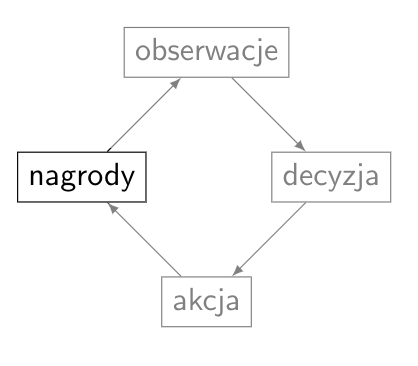
\includegraphics[width=.4\linewidth]{figures/learning_loop_4.png}}
			\vspace{7cm}
			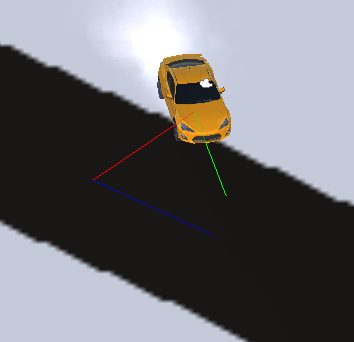
\includegraphics[width=\linewidth]{figures/rewards.png}
		\end{column}
	\end{columns}
	
\end{frame}
